% -*- root: ../../DAT2-A423_Project_Report.tex -*-
We started out by using the relatively simple LSB-method for hiding data in an image.
Specifically, we saved an image inside of another PNG-image.
While the differences in the image with and without the message-image were hardly noticeable to the human eye, we did find that comparing colour histograms of the two images revealed that there had in fact been made changes to it.
In an effort to diminish this problem, the graph-theoretical approach we implemented attempted to move pixels around in the image, rather than change their values.
This meant that colour histograms of the image before and after the message had been encoded should look very similar, almost identical.
Any changes would come from the unmatched pairs: the quantized DCT values used in the encoding that we did not find any interchangeable values for.
When this happened we were forced to change the individual values, which led to a change in the colour composition of the image.
Using this method, we expected the changes to be small enough so that it would not immediately draw attention to the image, if it was being subjected to a colour histogram.

\section{Changes to the Image}
To find out roughly how many of these forces there were in a given image, we used our programme to save different messages in different images.
The used five different message lengths were: 70, 140, 280, 560 and 1120 bytes.
Each message consisted of the ASCII characters A-Z repeated to fill out the message.
Each of these messages were encoded in four images with varying motives, but the same resolution (1920x1080).
The images can be seen in figure \ref{fig:four_test_images}.

We used a cartoon-like drawing of a cat to see how our software would work on an image that was not ideal for the JPEG format.
The landscape image contained many different colours and very complex patterns, which made it ideal for JPEG compression.
The same could be said for the tiger, but it contained larger areas of similar colours than the landscape did.
The image of the snowy forest road contained very few colour nuances, but was almost entirely made up of the luminance channel.
This led to a total of 20 tests as seen in table \ref{fig:forces_swaps}.

\begin{figure}[H]
    \centering
    \begin{subfigure}[b]{0.33\textwidth}
        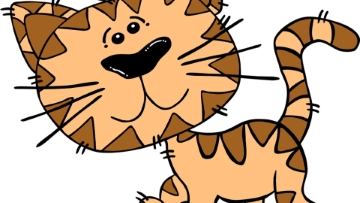
\includegraphics[width=\textwidth]{figures/cat}
            \caption{Cat image \citep{imgCat}}
    \end{subfigure}
    \begin{subfigure}[b]{0.33\textwidth}
            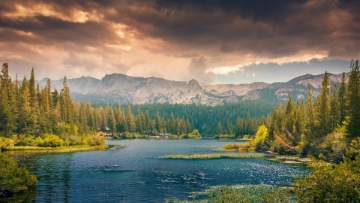
\includegraphics[width=\textwidth]{figures/landscape}
            \caption{Landscape image \citep{imgLandscape}}
    \end{subfigure}
    \begin{subfigure}[b]{0.33\textwidth}
            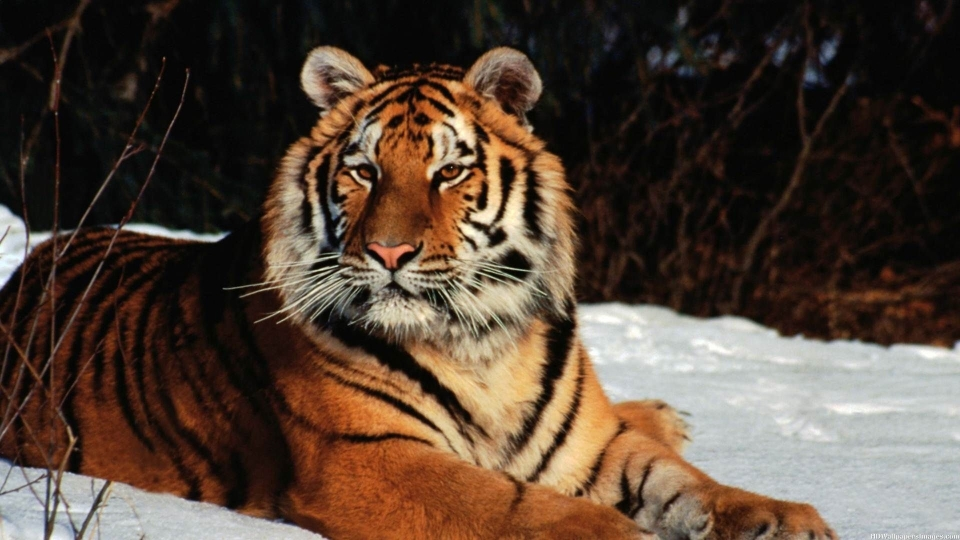
\includegraphics[width=\textwidth]{figures/tiger}
            \caption{Tiger image \citep{imgTiger}}
    \end{subfigure}
    \begin{subfigure}[b]{0.33\textwidth}
            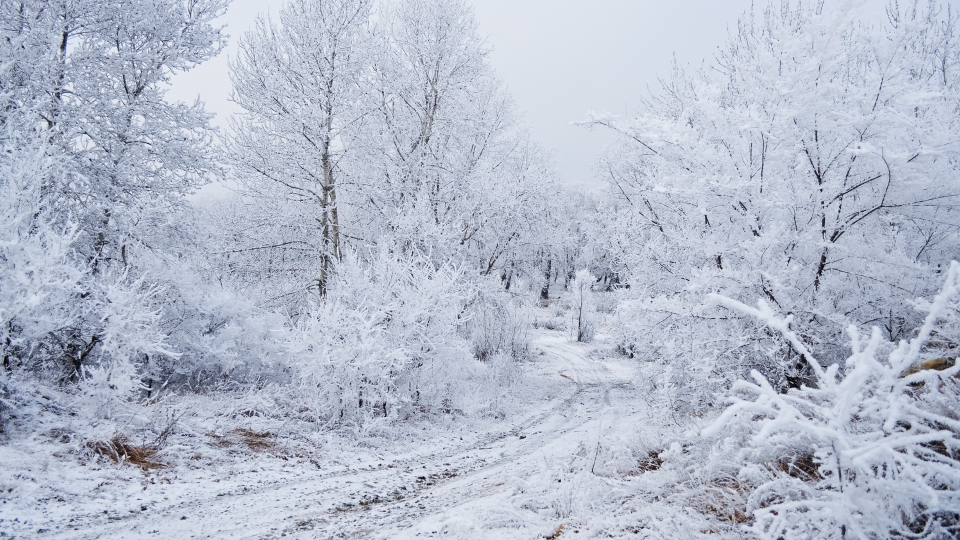
\includegraphics[width=\textwidth]{figures/snow}
            \caption{Snow image \citep{imgSnow}}
    \end{subfigure}
    \caption{The four images used for the tests in table \ref{fig:forces_swaps}}
    \label{fig:four_test_images}
\end{figure}

\begin{table}[H]
    \centering
	\caption{The percentages of values which the program swapped or forced. Since this was run with M = 4, about a fourth of the values already fit.}
    \label{fig:forces_swaps}
    \resizebox{0.7\textwidth}{!}{%
        \begin{tabular}{@{}lllll@{}}
            \textbf{Image}                      & \textbf{Message length} & \textbf{Swaps} & \textbf{Forces} & \textbf{Already fit} \\ \midrule
            \multirow{5}{*}{\textit{Cat}}       & 70                      & 56\%           & 19\%            & 26\%                 \\
                                                & 140                     & 58\%           & 18\%            & 24\%                 \\
                                                & 280                     & 65\%           & 12\%            & 23\%                 \\
                                                & 560                     & 65\%           & 11\%            & 24\%                 \\
                                                & 1120                    & 66\%           & 8\%             & 25\%                 \\ \midrule
            \multirow{5}{*}{\textit{Landscape}} & 70                      & 55\%           & 15\%            & 30\%                 \\
                                                & 140                     & 63\%           & 11\%            & 27\%                 \\
                                                & 280                     & 62\%           & 11\%            & 27\%                 \\
                                                & 560                     & 62\%           & 13\%            & 25\%                 \\
                                                & 1120                    & 63\%           & 12\%            & 25\%                 \\ \midrule
            \multirow{5}{*}{\textit{Tiger}}     & 70                      & 63\%           & 8\%             & 28\%                 \\
                                                & 140                     & 64\%           & 8\%             & 27\%                 \\
                                                & 280                     & 68\%           & 6\%             & 26\%                 \\
                                                & 560                     & 70\%           & 5\%             & 25\%                 \\
                                                & 1120                    & 72\%           & 4\%             & 24\%                 \\ \midrule
            \multirow{5}{*}{\textit{Snow}}      & 70                      & 53\%           & 21\%            & 26\%                 \\
                                                & 140                     & 58\%           & 13\%            & 29\%                 \\
                                                & 280                     & 66\%           & 8\%             & 26\%                 \\
                                                & 560                     & 67\%           & 8\%             & 25\%                 \\
                                                & 1120                    & 69\%           & 7\%             & 24\%                 \\ \bottomrule
        \end{tabular}
    }
\end{table}

As the table showed, some of the images required much fewer forces than others.
The main reason for this was that the changes in color within the area in which the message was encoded was different from image to image.
For example, the tiger performed much better than the other images, because it contained mostly the same colour in the area that contained the message.
When constructing the graph, we only added edges with a weigth under a certain threshold.
When the colours of an area were closer together, there would also be a higher concentration of edges with a smaller weight, which would lead to a larger graph.

\section{Size of the Graph}
It became apparent that a longer message required fewer forces. 
This made sense, seeing as a longer message meant a larger graph with more edges and therefore possible ways of swapping values.
During development of the programme we played around with the idea of using more vertices than what was required for the message, as we predicted it would mean fewer forces.
These predictions would seem to be correct, but we never implemented the idea for two reasons.

One, we were not entirely certain how to do it: should we just use twice as much as was actually needed?
This would lead to using much more than what was necessary with a longer message, since the improvement quickly diminishes with longer messages.
Instead it would make more sense to always use a certain minimum of values, so shorter messages could be encoded properly, but longer ones did not take too long to encode.
What were to happen if the image simply did not contain enough values then? 
Should the programme inform the user that they needed to use a larger image or attempt to encode the message with the vertices it could make?
What would this mean for the \lstinline|GetCapacity| method? 
Should it take into consideration these extra values or just ignore it entirely?
An entirely different approach would be to let the user decide themselves, how many values they wished the algorithm to use. 
Presenting this in a user-friendly way constituted a challenge in itself though.

The second reason we did not implement it was due to performance concerns.
Since our programme performed rather poorly during most of the development we considered it a very bad idea to construct a larger graph than we already were constructing.
Seeing as we managed to optimise the programme quite significantly, we could have properly implemented a solution regardless.

\section{Colour Histograms}
Actually comparing colour histograms from the two methods was not as trivial as one could have hoped.
Using the LSB-method only made immediately visible changes to the colour histograms if about a quarter of the image had data encoded in it.
When using an image of substantial size, a quarter of an image can hold a large amount of data. 
A 512x512 image for example can hold 196,604 bytes, when using the two least significant bits.
Encoding 40,000 bytes using our graph-theoretical (GT) programme was completely out of the question due to the complexity of the algorithm.
The longest message we tried encoding was just under 8960 bytes and took around half an hour on a decent desktop computer.
Running several test runs with different message lengths made it clear that the complexity of the programme made it infeasible to ever complete an encoding of this much data.

This made a direct comparison using realistic real-world images and messages impossible. 
The only real comparison we could make was between images containing different messages that used up every single available byte in the image.
Since the GT method became very time consuming with larger messages, we would need to use an image that was small enough that we could embed all bytes possible, without it taking too long to complete.
We ended up using an image with a resolution of 120x120 pixels.

\begin{figure}
    \centering
    \begin{subfigure}[b]{0.49\textwidth}
        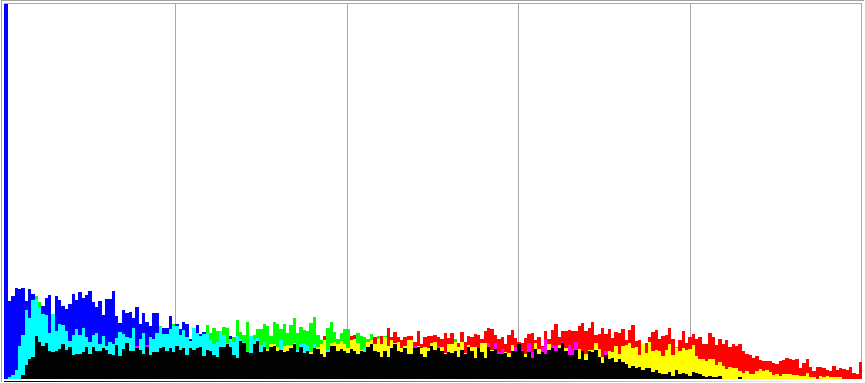
\includegraphics[width=\textwidth]{figures/tiger_smallHisto.png}
            \caption{Cover image}
            \label{fig:coverHisto}
    \end{subfigure}
    \begin{subfigure}[b]{0.49\textwidth}
            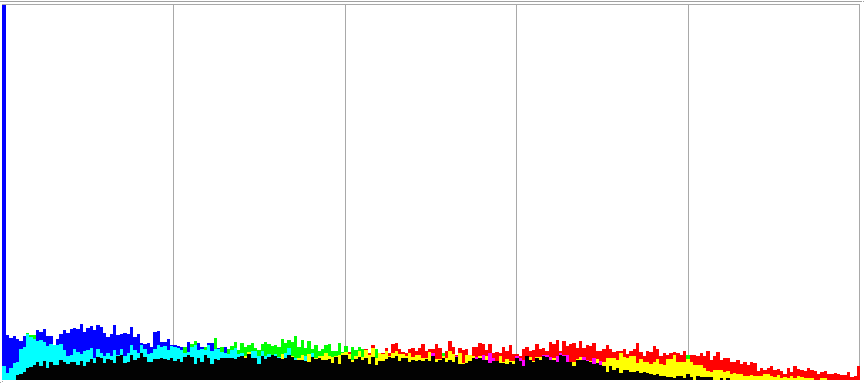
\includegraphics[width=\textwidth]{figures/gtOut2Histo.png}
            \caption{Cover image as JPEG}
            \label{fig:gt2Histo}
    \end{subfigure}
    \begin{subfigure}[b]{0.49\textwidth}
            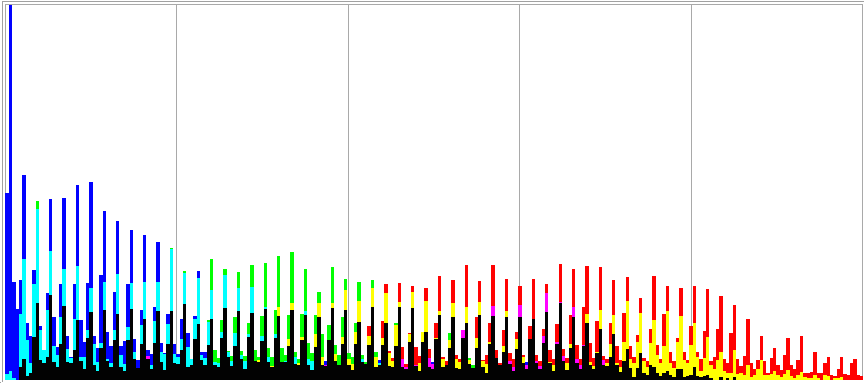
\includegraphics[width=\textwidth]{figures/lsbOutHisto.png}
            \caption{Stego image with message (LSB)}
            \label{fig:lsbHisto}
    \end{subfigure}
    \begin{subfigure}[b]{0.49\textwidth}
            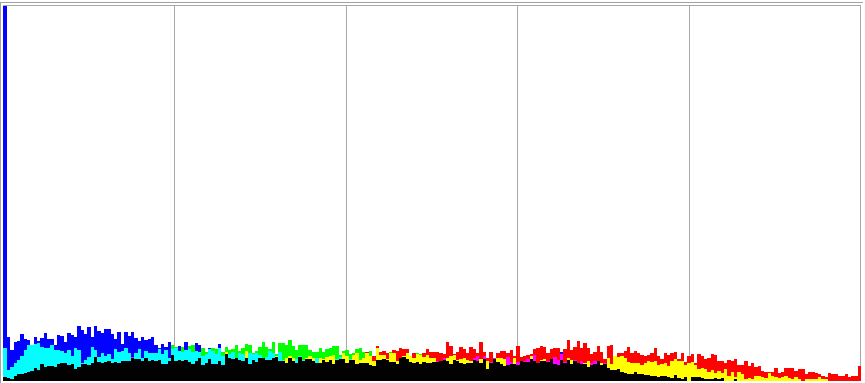
\includegraphics[width=\textwidth]{figures/gtOutHisto.png}
            \caption{Stego image with message (GT)}
            \label{fig:gtHisto}
    \end{subfigure}
    \caption{Histogram of a 120x120 px image}
    \label{fig:histogramsComparisons}
\end{figure}

In figure \ref{fig:histogramsComparisons} four histograms are shown.
Figures \ref{fig:coverHisto} and \ref{fig:gt2Histo} show the histogram of the original image and for the image encoded as JPEG without a message.
In figure \ref{fig:lsbHisto} and \ref{fig:gtHisto} the histograms of the images filled with a message using the LSB and GT methods respectively.
From these results it was clear that there was not much difference between the colour histograms of the image saved as JPEG with or without the message.
The image saved with LSB's histogram, however, clearly showed signs that the image had been tampered with.

The reason the histogram looked like that for the LSB image was because the bit-patterns of the encoded data became very clear in the histograms.
The bytes encoded in the images were the characters A-Z in ASCII repeated the capacity of the image had been reached.
A-Z in ASCII ranges from $65-90$, or in base two: $01000001_2-01011010_2$.
As the range was quite short, a lot of the higher order bits would rarely change, and those patterns became obvious in the histogram, as pixels ending in these patterns became more common.

The histogram in figure \ref{fig:lsbHisto} also showed how the LSB method changed images where a colour is very common.
The leftmost bar described pixels whose B-component is 0.
In the original cover image, this bar was much higher than the others, and therefore much more common in the image, but the LSB has made it so that those components now get spread out, which again becomes very obvious in the histogram.

\section{Euclidean Distance}
A different way of looking for changes in an image is by looking at their Euclidean distance.
This can be done by calculating the distance between the colour values of each pixel in two equally sized images.
The sum of all these distances can be used as measure of the change from one image to the other.
We used this same method for determining what changes were imposed on images of different size and format, when uploaded to various social media and image-sharing websites.
The images used for the method were the same as those previously used in the colour histogram tests.

Comparing the results of GT directly with the ones obtained from the LSB-method would be folly.
While the LSB-method might incur a smaller difference in the Euclidean distance it did not necessarily make it any better at hiding the information.
Comparing those two directly meant that we were looking at an image saved in the lossless PNG format and a file that not only had a message in it, but had also been compressed in a lossy way.
Therefore a comparison between the original and an image saved with our JPEG encoder, but containing no message, should yield a difference in euclidean distance as well.
The results of these tests can be seen in table \ref {fig:euclidean_distance}.

\begin{table}[]
	\centering
	\begin{tabular}{@{}lllll@{}}
		\toprule
		\textbf{Images}            & \textbf{All channels} & \textbf{R} & \textbf{G} & \textbf{B} \\ \midrule
		\textit{Original and LSB}  & 34671                 & 17098      & 16800      & 16824      \\
		\textit{Original and GT}   & 130389                & 71112      & 56972      & 71886      \\
		\textit{Original and JPEG} & 102460                & 56758      & 40707      & 57569      \\
		\textit{JPEG and GT}       & 79163                 & 42154      & 38833      & 43217     
	\end{tabular}
	\caption{Calculated euclidean distances for several combinations of images.}
	\label{fig:euclidean_distance}
\end{table}

It was clear that compressing the image with JPEG increased the euclidean distance between the two images.
But the distance between the JPEG image with a message and the one without it, was still larger than that of the LSB method and the original.
This was due to the fact that using the LSB of every pixel there was only the potential to change the value of each pixel by four.
With the GT method and an M value of four, means that each individual quantized value could also be changed by four. 
So why the big difference? 
We applied the change after the quantization step of JPEG encoding to avoid losing the data again, since the quantization step was what made JPEG encoding lossy.
This in turn meant that the small change of up to four was multiplied by the quantization table, when the image was shown and we calculated the distance.

But what did this actually mean for using the GT method to hide data?
Using euclidean distance to see if images had been tampered with, required that the intercepting party be in possession of both the original and the stego image.
This would indeed be possible if those sharing secret messages in images, were using cover images found on the internet and tampered with them.
It would not be all the difficult to reverse image search the internet to find what was probably the original cover image and measure the euclidean distance between the two images.
However, this would mean that any risk of being compromised by an outside party measuring euclidean distance, could be completely negated by simply using cover images that were not available to any intercepting parties.


Such a system could, however, check the histogram of the image, and discover abnormalities such as those the LSB method produces, as shown in figure \ref{fig:lsbHisto}.
Doing this would lead to very few useful results on images with messages hidden in them, using the GT programme.